%%%%%%%%%%%%  Generated using docx2latex.com  %%%%%%%%%%%%%%

%%%%%%%%%%%%  v2.0.0-beta  %%%%%%%%%%%%%%

\documentclass[12pt]{article}
\usepackage{amsmath}
\usepackage{latexsym}
\usepackage{amsfonts}
\usepackage[normalem]{ulem}
\usepackage{array}
\usepackage{amssymb}
\usepackage{graphicx}
\usepackage[backend=biber,
style=numeric,
sorting=none,
isbn=false,
doi=false,
url=false,
]{biblatex}\addbibresource{bibliography.bib}
\pagenumbering{gobble}
\usepackage{subfig}
\usepackage{wrapfig}
\usepackage{wasysym}
\usepackage{enumitem}
\usepackage{adjustbox}
\usepackage{ragged2e}
\usepackage[svgnames,table]{xcolor}
\usepackage{tikz}
\usepackage{longtable}
\usepackage{changepage}
\usepackage{setspace}
\usepackage{hhline}
\usepackage{multicol}
\usepackage{tabto}
\usepackage{float}
\usepackage{multirow}
\usepackage{makecell}
\usepackage{fancyhdr}
\usepackage[toc,page]{appendix}
\usepackage[hidelinks]{hyperref}
\usetikzlibrary{shapes.symbols,shapes.geometric,shadows,arrows.meta}
\tikzset{>={Latex[width=1.5mm,length=2mm]}}
\usepackage{flowchart}\usepackage[paperheight=11.0in,paperwidth=8.5in,left=1.0in,right=1.0in,top=0.39in,bottom=1.0in,headheight=1in]{geometry}
\usepackage[utf8]{inputenc}
\usepackage[T1]{fontenc}
\TabPositions{0.5in,1.0in,1.5in,2.0in,2.5in,3.0in,3.5in,4.0in,4.5in,5.0in,5.5in,6.0in,}

\urlstyle{same}


 %%%%%%%%%%%%  Set Depths for Sections  %%%%%%%%%%%%%%

% 1) Section
% 1.1) SubSection
% 1.1.1) SubSubSection
% 1.1.1.1) Paragraph
% 1.1.1.1.1) Subparagraph


\setcounter{tocdepth}{5}
\setcounter{secnumdepth}{5}


 %%%%%%%%%%%%  Set Depths for Nested Lists created by \begin{enumerate}  %%%%%%%%%%%%%%


\setlistdepth{9}
\renewlist{enumerate}{enumerate}{9}
		\setlist[enumerate,1]{label=\arabic*)}
		\setlist[enumerate,2]{label=\alph*)}
		\setlist[enumerate,3]{label=(\roman*)}
		\setlist[enumerate,4]{label=(\arabic*)}
		\setlist[enumerate,5]{label=(\Alph*)}
		\setlist[enumerate,6]{label=(\Roman*)}
		\setlist[enumerate,7]{label=\arabic*}
		\setlist[enumerate,8]{label=\alph*}
		\setlist[enumerate,9]{label=\roman*}

\renewlist{itemize}{itemize}{9}
		\setlist[itemize]{label=$\cdot$}
		\setlist[itemize,1]{label=\textbullet}
		\setlist[itemize,2]{label=$\circ$}
		\setlist[itemize,3]{label=$\ast$}
		\setlist[itemize,4]{label=$\dagger$}
		\setlist[itemize,5]{label=$\triangleright$}
		\setlist[itemize,6]{label=$\bigstar$}
		\setlist[itemize,7]{label=$\blacklozenge$}
		\setlist[itemize,8]{label=$\prime$}

\setlength{\topsep}{0pt}\setlength{\parindent}{0pt}
\renewcommand{\arraystretch}{1.3}


%%%%%%%%%%%%%%%%%%%% Document code starts here %%%%%%%%%%%%%%%%%%%%



\begin{document}
\begin{justify}
Deliverable\ 1\ \ \ \ \ \ \ \ \ \ \ \ \ \ \ \ \ \ \ \ \ \ \ \ \ \ \ \ \ \ \ \ \ \ \ \ \ \ \ \ \ \ \ \ \ \ \ \ \ Amandeep\ Kaur\ Khosa\ \ \ \ \ \ \ \ \ \ \ \ \ \ \ \ \ \ \ \ \ \ \ \ \ \ \ \ \ \ \ \ \ \ \ \ \ \ \ \ \ \ \ \ \ \ \ \ \ \ \ \ \ \ \ \ \ \ \ \ \ \ \ \ \ \ \ \ \ \ \ \ \ \ \ \ \ \ \ \ \ \ \ \ \ \ \ \ \ \ \ \ \ \ \ \ \ \ \ \ \ \ \ \ \ \ \ \ \ \ \ \ \ \ \      
\end{justify}\par

SOEN\ 6011\ \ \ \ \ \ \ \ \ \ \ \ \ \ \ \ \ \ \ \ \ \ \ \ \ \ \ \ \ \ \ \ \ \ \ \ \ \ \ \ \ \ \ \ \ \ \ \ \ \ \ \ \ \ \ \ \ \ \ \ \ \ \ \ \ \ \ \ \ \ \ \ \ \ \ \ \ \ \ \ \ \ \ \ \ \ \ \ \ \ \ \ \ \ \ \   40067608\par


\vspace{\baselineskip}
\textbf{Problem 1: - }Give a brief description, not exceeding one page, of your function, including the domain and co-domain of function, and the characteristics that make it unique. To ensure that you have attained sufficient background, Test 1 will have a problem related to your function.\par


\vspace{\baselineskip}
\textbf{Solution: - }My function ab$ \string^ $ x\par

This exponential function ab$ \string^ $ x means y increases exponentially as raising x. The initial quantity is given by the value that is easy to see (let x=0 and y=a left). Here value b is the growth factor. If we limit b to 0<b1, the function will increase.\par


\vspace{\baselineskip}
The graphs for the function are depicted below:\par



%%%%%%%%%%%%%%%%%%%% Figure/Image No: 1 starts here %%%%%%%%%%%%%%%%%%%%

\begin{figure}[H]
\advance\leftskip 0.0in		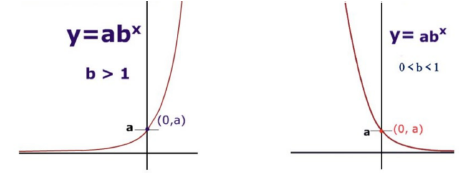
\includegraphics[width=5.67in,height=2.12in]{image1.PNG}
\end{figure}


%%%%%%%%%%%%%%%%%%%% Figure/Image No: 1 Ends here %%%%%%%%%%%%%%%%%%%%

\par


\begin{adjustwidth}{0.5in}{0.0in}
\textit{Exponential growth \tabto{3.99in} Exponential decay}\par

\end{adjustwidth}


\vspace{\baselineskip}
\vspace{\baselineskip}
\vspace{\baselineskip}

%%%%%%%%%%%%%%%%%%%% Table No: 1 starts here %%%%%%%%%%%%%%%%%%%%


\textbf{Domain: - }{[ $\infty$ } to { $\infty$ ]} \par
\textbf{Range: - }[0 to { $\infty$ ]} \par

\vspace{\baselineskip}
\vspace{\baselineskip}

\textbf{Characteristics}: \par 

\begin{itemize}
    \item The exponential growth as shown above, is when b>1.\par
    \item If 0 < b < 1, there is an exponential decay.\par
	\item The graph does not have a constant rate of change having constant ratios.\par

	\item This graph is growing by common factors over equal intervals.
\end{itemize}\par


\vspace{\baselineskip}
\vspace{\baselineskip}
\vspace{\baselineskip}
\vspace{\baselineskip}
\vspace{\baselineskip}\textbf{Problem 2: - }Express requirements of your function based on the style given in the ISO/IEC/IEEE 29148 Standard. Associate each requirement with a unique identifier. Make any assumptions explicit.\par


\vspace{\baselineskip}\begin{justify}
\textbf{Solution: - Requirements}
\end{justify}\par




\begin{adjustwidth}{0.25in}{0.0in}
\begin{justify}
 First Requirement
\end{justify}\par

\end{adjustwidth}



\begin{adjustwidth}{0.49in}{0.0in}
\begin{justify}
ID = FR1
\end{justify}\par

\end{adjustwidth}



\begin{adjustwidth}{0.49in}{0.0in}
\begin{justify}
Type = Functional Requirements
\end{justify}\par

\end{adjustwidth}



\begin{adjustwidth}{0.49in}{0.0in}
\begin{justify}
Version = 1.0
\end{justify}\par

\end{adjustwidth}



\begin{adjustwidth}{0.49in}{0.0in}
\begin{justify}
Difficulty = Hard
\end{justify}\par

\end{adjustwidth}



\ \ \ \ \ \ \ \ \ Description = The input should be a real number\par











\begin{adjustwidth}{0.35in}{0.0in}
\begin{justify}
Second Requirement
\end{justify}\par

\end{adjustwidth}



\begin{adjustwidth}{0.49in}{0.0in}
\begin{justify}
ID = FR2
\end{justify}\par

\end{adjustwidth}



\begin{adjustwidth}{0.49in}{0.0in}
\begin{justify}
Type = Functional Requirements
\end{justify}\par

\end{adjustwidth}



\begin{adjustwidth}{0.49in}{0.0in}
\begin{justify}
Version = 1.0
\end{justify}\par

\end{adjustwidth}



\begin{adjustwidth}{0.49in}{0.0in}
\begin{justify}
Difficulty = Hard
\end{justify}\par

\end{adjustwidth}



\begin{adjustwidth}{0.49in}{0.0in}
\begin{justify}
Description = For real numbers ranging between [-\textcolor[HTML]{545454}{ $\infty$ } to +\textcolor[HTML]{545454}{ $\infty$ ]}, the results should always be in the range of [0, \textcolor[HTML]{545454}{$\infty$ }]
\end{justify}\par

\end{adjustwidth}







\begin{adjustwidth}{0.25in}{0.0in}
\begin{justify}
 Third Requirement
\end{justify}\par

\end{adjustwidth}



\begin{adjustwidth}{0.49in}{0.0in}
\begin{justify}
ID = FR3
\end{justify}\par

\end{adjustwidth}



\begin{adjustwidth}{0.49in}{0.0in}
\begin{justify}
Type = Functional Requirements
\end{justify}\par

\end{adjustwidth}



\begin{adjustwidth}{0.49in}{0.0in}
\begin{justify}
Version = 1.0
\end{justify}\par

\end{adjustwidth}



\begin{adjustwidth}{0.49in}{0.0in}
\begin{justify}
Difficulty = Hard
\end{justify}\par

\end{adjustwidth}



\ \ \ \ \ \ \ \ \ Description = The output should allow negative numbers\par



\begin{adjustwidth}{0.35in}{0.0in}
\begin{justify}
Fourth Requirement
\end{justify}\par

\end{adjustwidth}



\begin{adjustwidth}{0.49in}{0.0in}
\begin{justify}
ID = FR4
\end{justify}\par

\end{adjustwidth}



\begin{adjustwidth}{0.49in}{0.0in}
\begin{justify}
Type = Functional Requirements
\end{justify}\par

\end{adjustwidth}



\begin{adjustwidth}{0.49in}{0.0in}
\begin{justify}
Version = 1.0
\end{justify}\par

\end{adjustwidth}



\begin{adjustwidth}{0.49in}{0.0in}
\begin{justify}
Difficulty = Easy
\end{justify}\par

\end{adjustwidth}



\ \ \ \ \ \ \ \ \ Description = The output should show infinite numbers\par



\vspace{\baselineskip}

\vspace{\baselineskip}

\vspace{\baselineskip}
\printbibliography
\end{document}